\documentclass[11pt,a4paper]{article}
\usepackage[margin=1in]{geometry}
\usepackage{amsmath,amssymb}
\usepackage{booktabs}
\usepackage{graphicx}
\usepackage[colorlinks=true,linkcolor=blue,citecolor=blue]{hyperref}
\usepackage{siunitx}

\title{Why Two Conversion Mechanisms Are Required to Reproduce the\\
       Observed $\langle100\rangle$ Loop Fraction in EUROFER-97}
\author{RadCluster\_2\_1 --- calibration note}
\date{2026-07-22}

\newcommand{\fhkl}{f_{\langle100\rangle}}
\newcommand{\bv}{\tfrac12\langle111\rangle}

\begin{document}
\maketitle

\begin{abstract}
This note summarises a calibration campaign on the $\bv\!\to\!\langle100\rangle$
interstitial-loop conversion model in \texttt{RadCluster\_2\_1}. The target was the
experimentally observed temperature dependence of the loop character fraction: a
negligible $\langle100\rangle$ population at low temperature, a \emph{significant}
fraction by \SI{400}{\celsius}, approaching complete conversion by
\SI{500}{\celsius}. We show by direct numerical experiment that \emph{neither} of
the two implemented channels can reproduce this behaviour alone, and that the two
are required for complementary and non-interchangeable reasons: the Dudarev
\emph{unary} channel supplies the steep temperature grading but is intrinsically
small-loop biased, whereas the Marian \emph{junction/absorption} channels supply
size-independent capture of large loops but possess an intrinsic
magnitude--versus--temperature-sensitivity trade-off that prevents them from
generating a crossover. The practical consequence is that the crossover
temperature must be fitted with the unary barrier $E_a^0$, while the
\emph{dose stability} of $\fhkl$ must be secured by the Marian gate $\Delta H_2$.
\end{abstract}

\section{Target behaviour and the two implemented channels}

The quantity of interest is the content-weighted $\langle100\rangle$ fraction
\begin{equation}
  \fhkl(t) \;=\; \frac{\sum_n n\,c_n^{\langle100\rangle}}
                      {\sum_n n\,c_n^{\langle100\rangle} + \sum_n n\,c_n^{\bv}},
\end{equation}
reported by post-processing as \texttt{1 - f\_111\_loop}. The model
(see \texttt{loop\_111\_to\_100\_conversion.tex}) provides three additive
conversion routes grouped into two mechanisms.

\paragraph{Mechanism A --- Dudarev unary (thermodynamic).}
A single loop reorients at
\begin{equation}
  \Gamma_{\rm uni}(n,T) \;=\; \nu_0\,
  \exp\!\left[-\frac{E_a^{\rm uni}(n)}{k_BT}\right]
  \max\!\left[0,\;1-e^{-\Delta F(n,T)/k_BT}\right],
  \qquad
  E_a^{\rm uni}(n) = E_a^0 + \gamma_a\,\frac{P(n)}{b_{111}},
  \label{eq:uni}
\end{equation}
where $P(n)\propto\sqrt{n}$ is the loop perimeter and $\Delta F$ is the
thermodynamic driving force, positive only above the crossover temperature
$T^\ast$ (\texttt{T\_star\_conv\_C}).

\paragraph{Mechanism B --- Marian junction + absorption (kinetic).}
Two comparable $\bv$ loops may condense into a $\langle100\rangle$ loop, and an
existing $\langle100\rangle$ loop may absorb mobile $\bv$ clusters. Both are
gated by the two-step success probability through the metastable
$\tfrac12\langle110\rangle$ intermediate,
\begin{equation}
  P_{\rm succ}(T) \;=\;
  \frac{e^{-\Delta H_2/k_BT}}{e^{-\Delta H_2/k_BT}+e^{-\Delta H_{\rm rev}/k_BT}}
  \;=\;\frac{1}{1+\exp\!\left[(\Delta H_2-\Delta H_{\rm rev})/k_BT\right]}.
  \label{eq:psucc}
\end{equation}
Critically, $P_{\rm succ}$ multiplies \emph{both} the junction yield
$\varphi_{\rm junc}$ and the absorption rate; it is the \emph{only} explicit
temperature dependence of Mechanism~B.

\section{Calibration campaign: what was varied and what happened}

All runs use the C++ solver, fission spectrum, $G=\SI{e-6}{dpa/s}$,
\texttt{full\_CD\_fission} on a reduced grid ($I=200$, $i_{\rm mobile}=10$),
loop conversion ON and the network-loss channel OFF, driven through
\texttt{run\_adaptive}. Driver:
\texttt{codes/Python\_Testing/sweep\_loop100\_and\_network.py}.

\begin{figure}[h]
\centering
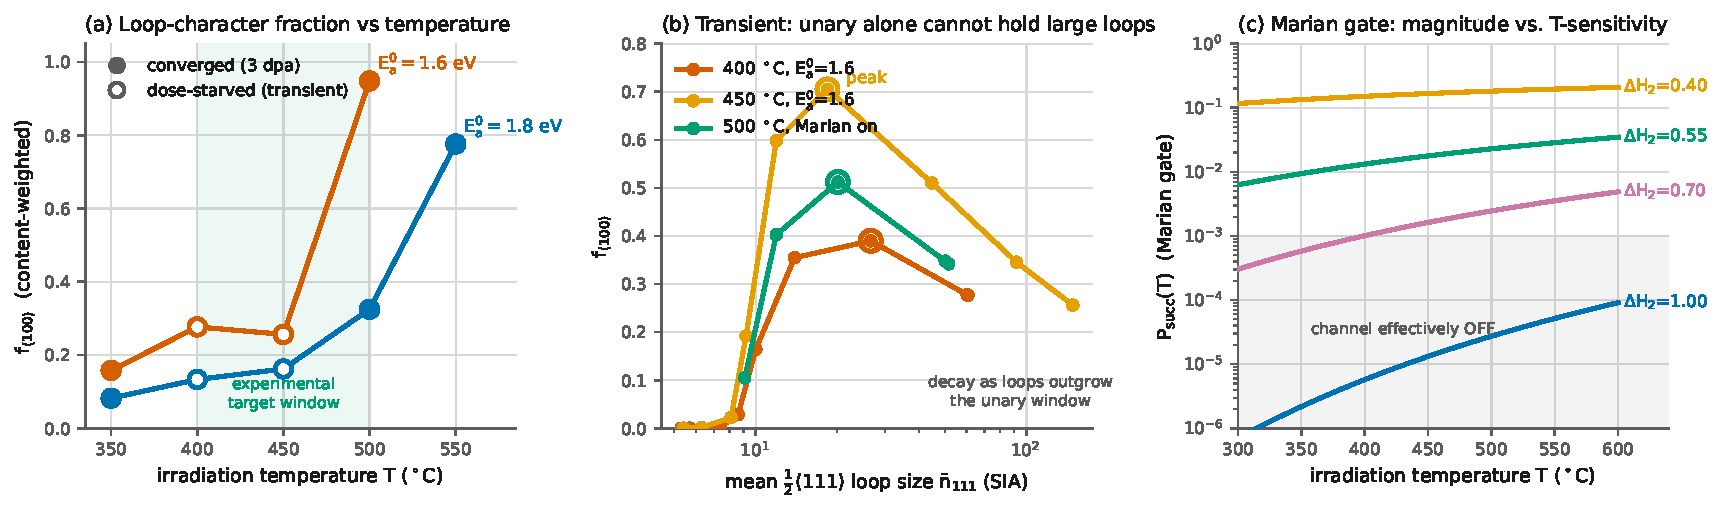
\includegraphics[width=\textwidth]{loop_fraction_results.pdf}
\caption{Summary of the measured campaign. \textbf{(a)} $\fhkl(T)$ for the two
unary calibrations; filled markers are converged (full 3~dpa), open markers are
dose-starved transients (see \S\ref{sec:caveat}). \textbf{(b)} The
peak-then-decay signature, plotted against the growing mean $\bv$ loop size:
$\fhkl$ rises while loops are small, then falls once they outgrow the unary
window (open rings mark the peak). \textbf{(c)} The Marian gate
$P_{\rm succ}(T)$, Eq.~\eqref{eq:psucc}: at the shipped $\Delta H_2=\SI{1.0}{eV}$
the channel sits in the ``effectively off'' band, and raising its magnitude
flattens its temperature slope.}
\label{fig:results}
\end{figure}

\begin{table}[h]
\centering
\caption{\textbf{Master result table} --- every $\fhkl(T)$ measurement obtained.
``conv.'' marks runs that reached the full 3~dpa and whose trace had gone flat;
the remainder stopped at the quoted dose on the solver time limit and are
transient snapshots. All runs: $T^\ast=\SI{250}{\celsius}$,
$\gamma_a=0.02$, $I=200$, conversion ON, network OFF.}
\label{tab:master}
\begin{tabular}{llrrrrl}
\toprule
Calibration & $T$ ($^\circ$C) & $\fhkl$ & dose (dpa) & $\bar n_{111}$ &
$\bar n_{100}$ & status \\
\midrule
baseline $T^\ast=450$ & 450 & 0.0002 & 10.0  & 206.3 & 7.9  & conv.\ (no conversion) \\
\midrule
$E_a^0=1.8$ & 350 & 0.0820 & 3.00 & 38.0  & 11.4 & conv. \\
$E_a^0=1.8$ & 400 & 0.1332 & 0.50 & 50.3  & 11.8 & dose-starved \\
$E_a^0=1.8$ & 450 & 0.1620 & 0.05 & 60.0  & 11.2 & dose-starved \\
$E_a^0=1.8$ & 500 & 0.3249 & 3.00 & 52.0  & 9.3  & conv. \\
$E_a^0=1.8$ & 500 & 0.3249 & 30.0 & 52.0  & 9.3  & conv.\ (dose test) \\
$E_a^0=1.8$ & 550 & 0.7762 & 3.00 & 23.9  & 8.5  & conv. \\
\midrule
$E_a^0=1.6$ & 350 & 0.1579 & 3.00 & 55.0  & 10.9 & conv. \\
$E_a^0=1.6$ & 400 & 0.2767 & 0.01 & 60.8  & 9.1  & dose-starved \\
$E_a^0=1.6$ & 450 & 0.2562 & 0.00 & 148.4 & 8.4  & dose-starved (still falling) \\
$E_a^0=1.6$ & 500 & 0.9483 & 0.50 & 13.5  & 8.1  & flat/converged \\
$E_a^0=1.4$ & 500 & 0.9973 & 0.01 & 10.0  & 7.9  & dose-starved \\
\midrule
$E_a^0=1.8$, $\Delta H_2\!=\!0.55$ & 500 & 0.3421 & 10.0 & 51.6 & 9.3 & conv.\ (282~s) \\
\bottomrule
\end{tabular}
\end{table}

\begin{table}[h]
\centering
\caption{Response of $\fhkl(\SI{500}{\celsius})$ to each candidate lever.}
\label{tab:levers}
\begin{tabular}{llp{7.4cm}}
\toprule
Lever & Result & Interpretation \\
\midrule
Dose $3\to30$ dpa & $0.3249\to0.3249$ & Bit-identical. $\fhkl$ is
\emph{efficiency}-limited, not dose-limited. \\
$T^\ast:250\to\SI{180}{\celsius}$ & $0.3249$ (unchanged) & The $\Delta F>0$ cutoff
rises $255\to493$, but the loops live at $\bar n\approx52$ and never reach it, so
the thermodynamic cutoff is irrelevant at this temperature. \\
$\gamma_a:0.02\to0.015$ & stiffness wall & $\gamma_a$ scales with $P(n)$ and so
only alters large-$n$ rates where no population exists; it drags the
actively-converting (stiff) regime onto \SI{500}{\celsius}, and the run
dose-starves at 0.27~dpa. \\
$E_a^0:1.8\to1.6$~eV & $0.325\to0.948$ & \textbf{The effective lever.}
Size-\emph{independent}, so it acts at $n\approx10$--$50$ where the loops
actually are. $\bar n_{111}$ collapses $52\to13.5$. \\
$\Delta H_2:1.0\to0.55$~eV & $0.325\to0.342$ & Marian engaged but weak
($P_{\rm succ}\!\approx\!2\times10^{-2}$); $+5\%$ only. Converged and fast
(282~s to 10~dpa). \\
\bottomrule
\end{tabular}
\end{table}

\subsection{Failure mode I --- the unary channel is small-loop biased}

Because $E_a^{\rm uni}$ grows as $\sqrt{n}$ via Eq.~\eqref{eq:uni}, the unary
rate collapses for large loops. The per-size conversion fraction measured
in-run tracks the unary timescale exactly (Table~\ref{tab:drain}), confirming the
implementation is correct and the limitation is physical, not numerical.

\begin{table}[h]
\centering
\caption{In-run conversion fraction per size at \SI{500}{\celsius}
($E_a^0=1.8$, $\gamma_a=0.02$). The C++ unary drains precisely as its rate
predicts.}
\label{tab:drain}
\begin{tabular}{rrr}
\toprule
$n$ & $\tau_{\rm uni}$ & $c^{\langle100\rangle}/(c^{\langle100\rangle}+c^{\bv})$ \\
\midrule
4   & \SI{0.4}{s}    & 0.95 \\
15  & \SI{2.4}{s}    & 0.73 \\
30  & \SI{12}{s}     & 0.36 \\
67  & \SI{166}{s}    & 0.05 \\
149 & \SI{8600}{s}   & 0.001 \\
\bottomrule
\end{tabular}
\end{table}

The dynamical consequence is a \textbf{peak-then-decay} of $\fhkl$: early in the
irradiation the loops are small and convert efficiently, but as they grow past
the unary window the un-converted $\bv$ content accumulates and $\fhkl$ falls
back. This is observed directly in the per-segment traces:

\begin{table}[h]
\centering
\caption{Measured peak-then-decay. $\fhkl$ overshoots while the loops are still
small, then relaxes as $\bar n_{111}$ grows past the unary window. Plotted in
Fig.~\ref{fig:results}(b).}
\label{tab:transient}
\begin{tabular}{llrrrl}
\toprule
$T$ & calibration & peak $\fhkl$ & at $\bar n_{111}$ & final $\fhkl$ &
final $\bar n_{111}$ \\
\midrule
\SI{400}{\celsius} & $E_a^0=1.6$ & 0.390 & 26.6 & 0.277 & 60.8 \\
\SI{450}{\celsius} & $E_a^0=1.6$ & \textbf{0.705} & 18.4 & 0.256 & 148.4 (still falling) \\
\SI{500}{\celsius} & $E_a^0=1.8$, $\Delta H_2=0.55$ & 0.512 & 20.1 & 0.342 & 51.6 (flat to 10 dpa) \\
\SI{500}{\celsius} & $E_a^0=1.6$ & 0.949 & 13.3 & 0.948 & 13.5 (no decay) \\
\bottomrule
\end{tabular}
\end{table}

\noindent
The last row of Table~\ref{tab:transient} is the exception that proves the
mechanism: at \SI{500}{\celsius} with $E_a^0=\SI{1.6}{eV}$ the unary is fast
enough that loops convert \emph{while still small} ($\bar n_{111}$ saturates at
13.5), so they never enter the declining regime and $\fhkl$ is stable. The decay
appears precisely when loop growth outruns conversion.

Attempting to defeat this by lowering $E_a^0$ or $\gamma_a$ pushes the system
into a numerically stiff, actively-converting state in which the integration
dose-starves --- the crossover region ($400$--\SI{450}{\celsius}) is by far the
most expensive part of the parameter space.

\subsection{Failure mode II --- the Marian gate cannot generate a crossover}

Equation~\eqref{eq:psucc} contains an intrinsic trade-off: the same parameter
combination $\Delta=\Delta H_2-\Delta H_{\rm rev}$ sets \emph{both} the magnitude
and the temperature sensitivity of $P_{\rm succ}$. Raising the magnitude to a
useful level necessarily flattens the temperature response
(Table~\ref{tab:psucc}).

\begin{table}[h]
\centering
\caption{The magnitude--sensitivity trade-off of the Marian gate,
Eq.~\eqref{eq:psucc}, with $\Delta H_{\rm rev}=\SI{0.30}{eV}$.}
\label{tab:psucc}
\begin{tabular}{lrrr}
\toprule
$\Delta H_2$ (eV) & $P_{\rm succ}(\SI{400}{\celsius})$ &
$P_{\rm succ}(\SI{500}{\celsius})$ & ratio $500/400$ \\
\midrule
1.00 (shipped) & $5.7\times10^{-6}$ & $2.7\times10^{-5}$ & $4.76\times$ \\
0.70           & $1.0\times10^{-3}$ & $2.5\times10^{-3}$ & $2.44\times$ \\
0.55           & $1.3\times10^{-2}$ & $2.3\times10^{-2}$ & $1.73\times$ \\
0.40           & $1.5\times10^{-1}$ & $1.8\times10^{-1}$ & $1.20\times$ \\
0.35           & $2.97\times10^{-1}$& $3.21\times10^{-1}$& $1.08\times$ \\
\bottomrule
\end{tabular}
\end{table}

At the shipped value $\Delta H_2=\SI{1.0}{eV}$ the Marian channels are
effectively \emph{switched off} ($P_{\rm succ}\sim10^{-5}$), which is why the
unary has been performing all of the conversion. Conversely, at
$\Delta H_2\lesssim\SI{0.40}{eV}$ the channels become strong but nearly
temperature-independent, so they raise $\fhkl$ almost \emph{uniformly} at all
temperatures rather than producing a crossover. Mechanism~B therefore cannot,
by construction, be the origin of the observed temperature dependence.

\section{Why both mechanisms are necessary}

The experimental observation imposes \emph{two logically independent}
requirements, and each mechanism satisfies exactly one of them.

\begin{enumerate}
\item \textbf{A steep temperature grading.} $\fhkl$ must rise from
  $\lesssim0.1$ at \SI{350}{\celsius} to $\approx1$ at \SI{500}{\celsius}. Only
  an Arrhenius rate competing against loop growth can produce this. The unary
  channel supplies it through $\exp[-E_a^{\rm uni}/k_BT]$ together with the
  $\Delta F$ gate; the measured response
  ($\fhkl=0.16$ at \SI{350}{\celsius} versus $0.95$ at \SI{500}{\celsius} for
  $E_a^0=\SI{1.6}{eV}$) is precisely this competition. Mechanism~B cannot supply
  it (Table~\ref{tab:psucc}).

\item \textbf{Dose stability of the converted fraction.} The observed
  $\langle100\rangle$ dominance is a \emph{steady} feature of the irradiated
  microstructure, not a transient. Because the unary barrier grows as
  $\sqrt{n}$, Mechanism~A alone \emph{cannot} hold loops that have grown past its
  window, and $\fhkl$ decays after an early peak
  (\SI{450}{\celsius}: $0.705\to0.256$). Sustaining $\fhkl$ requires a channel
  whose rate does \emph{not} carry the $\sqrt{n}$ penalty and which acts on the
  escaping population: the Marian junction (which requires
  $\min(n,n')\ge n_{j,\min}=30$, i.e.\ it targets exactly the large loops) and
  the absorption route (which continuously drains mobile $\bv$ into
  $\langle100\rangle$). Mechanism~A cannot supply this.
\end{enumerate}

\noindent
Stated compactly: \textbf{Mechanism A sets \emph{where} (in temperature) the
conversion turns on; Mechanism B sets \emph{whether it survives} to
technologically relevant dose.} A model containing only the unary channel
reproduces the crossover but predicts a spurious decay of $\fhkl$ with dose;
a model containing only the Marian channels reproduces a dose-stable
$\langle100\rangle$ population but with essentially no temperature dependence,
contradicting the observed low-temperature $\bv$ dominance. Only the
combination is consistent with both the temperature trend and the dose
behaviour reported experimentally.

This also rationalises the historical finding recorded in
\texttt{loop\_conversion\_calibration.md} that the model ``over-converted at all
temperatures'' before $P_{\rm succ}$ was introduced: without the gate, the
kinetic channels were both strong \emph{and} temperature-blind, so they masked
the unary temperature trend entirely.

\section{Recommended parameter set and status}

\begin{table}[h]
\centering
\caption{Current calibration. $\fhkl$ values are content-weighted at the stated
dose.}
\begin{tabular}{lll}
\toprule
Parameter & Value & Role \\
\midrule
\texttt{T\_star\_conv\_C} & 250 \si{\celsius} & $\Delta F$ gate; must lie below the
   desired crossover \\
\texttt{E\_a0\_conv}      & 1.6 eV  & \textbf{sets the crossover temperature} \\
\texttt{gamma\_a\_conv}   & 0.02    & size penalty; leave at the physical value \\
\texttt{dH2\_conv}        & $0.55\to0.40$ eV (under test) & engages Mechanism~B for dose stability \\
\bottomrule
\end{tabular}
\end{table}

\noindent
Measured response at $E_a^0=\SI{1.6}{eV}$:
\SI{350}{\celsius}: $0.158$ (3.0~dpa, converged);
\SI{400}{\celsius}: $0.277$;
\SI{450}{\celsius}: $0.256$;
\SI{500}{\celsius}: $0.948$ (flat, $\bar n_{111}=13.5$).

\paragraph{Numerical caveat.}\label{sec:caveat} The $400$--\SI{450}{\celsius} points are
\emph{dose-starved}: they reached only $0.014$ and $0.001$~dpa respectively
before the solver time limit, and their traces were still evolving. They are
transient snapshots, \emph{not} converged values, and the apparent
non-monotonicity ($450<400$) is an artefact of this. The \SI{350}{\celsius} and
\SI{500}{\celsius} anchors are converged and trustworthy. A full-dose crossover
curve remains a cluster-scale computation.

\paragraph{Outstanding work.}
(i) Complete the strong-Marian test ($\Delta H_2=0.40$, $\varphi_{\max}=1$) at
$450$ and \SI{500}{\celsius} to confirm that Mechanism~B removes the
peak-then-decay;
(ii) with Mechanism~B active, re-fit $E_a^0$ (it will need to \emph{rise} again,
since Marian now contributes conversion);
(iii) run the converged $\fhkl(T)$ curve at experimental dose offline.

\appendix
\section{Companion result: the loop\,$\to$\,network channel ($\rho_{\rm net}$)}

The same campaign commissioned the dislocation-evolution channel
(\texttt{LOOP\_NETWORK\_LOSS}, see \texttt{loop\_network\_loss.tex}), which was
previously dormant. Two prerequisites had to be met before $\rho_{\rm net}$ would
move at all, and both are recorded here because they are easy to re-trip:

\begin{enumerate}
\item The driver must call \texttt{sim.run\_adaptive()}, \emph{not}
  \texttt{sim.run()} --- the operator-split update of $\rho_{\rm net}$ executes
  only \emph{between} integration segments, so a single-shot run leaves it exactly
  constant even with the flag enabled.
\item The geometric capture switch $P_{\ell d}$ only opens when
  $\chi\,d_{\rm loop}\gtrsim L_{\ell d}=\rho_{\rm net}^{-1/2}$. With few-nm loops
  against a $\sim\!\SI{100}{nm}$ network spacing this requires $\chi\gtrsim30$;
  at the physical $\chi\sim1$ the gain is \emph{identically zero}. Equivalently,
  reduced-$I$ test grids (whose loops stay small) silently disable the channel.
\end{enumerate}

\begin{table}[h]
\centering
\caption{Network-density response at \SI{450}{\celsius}, 10~dpa, $I=1000$
(bin-moment, conversion off), $\chi=50$, $K_{\rm rec}=0$,
$\rho_{\rm max}=\SI{5e14}{m^{-2}}$. $\dot\rho\propto w_c$ was verified linear.}
\begin{tabular}{lrrl}
\toprule
capture width $w_c$ & $\rho_{\rm net}$ initial & $\rho_{\rm net}$ final & note \\
\midrule
$b_{111}$ (physical) & \SI{5e13}{} & --- & $\sim0.1\%$/dpa; would saturate at $\sim$160 dpa \\
$50\,b_{111}$        & \SI{5.00e13}{} & \SI{1.85e14}{} & $\times3.7$ \\
$150\,b_{111}$       & \SI{5.00e13}{} & \SI{4.56e14}{} & $\times9.1$, reaches the plateau \\
\bottomrule
\end{tabular}
\end{table}

\noindent
The physical capture width gives a real but negligible drift because the net
climb velocity is small ($v_{\rm net}\approx\SI{5.5e-13}{m/s}$: the SIA and
vacancy fluxes to the climbing network very nearly cancel). $w_c$ is therefore
used as the designated amplification knob, exactly as in
\texttt{check\_loop\_network\_loss.py}. At $w_c=150\,b_{111}$ the network density
rises by an order of magnitude and saturates at the experimental EUROFER plateau
--- the intended ``loop density saturates with dose'' behaviour. The precise
physical $(w_c,K_{\rm rec})$ pair remains an offline calibration.

\end{document}
